\documentclass[xcolor={dvipsnames},aspectratio=169,10pt]{beamer}

% chktex-file 41

% check for obsoleted LaTeX packages
\usepackage[l2tabu,orthodox]{nag}

% utility packages
\usepackage{etoolbox}
\usepackage{xifthen}
\usepackage{xpatch}
\usepackage{adjustbox}

% better text justifying
\usepackage{microtype}
% justify text inside list environment
% Ref: http://liam0205.me/2017/04/11/justifying-in-beamer-s-lists/
\usepackage{ragged2e}
\makeatletter
\xpatchcmd{\itemize}{\raggedright}{\justifying}{}{}
\xpatchcmd{\beamer@enum@}{\raggedright}{\justifying}{}{}
\xpatchcmd{\@@description}{\raggedright}{\justifying}{}{}
\makeatother

% math related packages
\usepackage{amsmath}
\usepackage{amssymb}
\let\emptyset\varnothing%
\usepackage{amsfonts}
\usepackage{mathrsfs}
\usepackage{latexsym}
\usepackage{bm}
\usepackage{fancynum}

% equation style
\newcommand{\setdisplayskip}{%
  \abovedisplayskip=0.25\baselineskip plus 0.05\baselineskip minus 0.125\baselineskip% chktex 1
  \abovedisplayshortskip=0pt plus 0.075\baselineskip% chktex 1
  \belowdisplayskip=0.25\baselineskip plus 0.05\baselineskip minus 0.125\baselineskip% chktex 1
  \belowdisplayshortskip=0.15\baselineskip plus 0.075\baselineskip minus 0.075\baselineskip% chktex 1
}
\apptocmd\Huge{\setdisplayskip}{}{}
\apptocmd\huge{\setdisplayskip}{}{}
\apptocmd\LARGE{\setdisplayskip}{}{}
\apptocmd\Large{\setdisplayskip}{}{}
\apptocmd\large{\setdisplayskip}{}{}
\apptocmd\normalsize{\setdisplayskip}{}{}
\apptocmd\small{\setdisplayskip}{}{}
\apptocmd\footnotesize{\setdisplayskip}{}{}
\apptocmd\scriptsize{\setdisplayskip}{}{}
\apptocmd\tiny{\setdisplayskip}{}{}

% figure related packages
\usepackage{graphicx}
\usepackage{tikz}
\usetikzlibrary{backgrounds,calc,decorations.pathreplacing,fit,matrix,patterns,positioning,shapes,shapes.multipart}
\usepackage{pgfplots}
\pgfplotsset{compat=1.16}
\usepackage[outline]{contour}
\contourlength{1.8pt}
\usepackage{pifont}
\makeatletter
% Ref: https://tex.stackexchange.com/a/62273
\newenvironment{customlegend}[1][]{%
  \begingroup
  \csname pgfplots@init@cleared@structures\endcsname
  \pgfplotsset{#1}
  \def\addlegendimage{\csname pgfplots@addlegendimage\endcsname}
  \def\addlegendentry{\csname pgfplots@addlegendentry\endcsname}
}{%
  \csname pgfplots@createlegend\endcsname
  \endgroup
}%
\makeatother

% table related packages
\usepackage{array}
\usepackage{tabu}
\usepackage{booktabs}
\usepackage{multirow}
\newcommand{\tabincell}[2]{\begin{tabular}{@{}#1@{}}#2\end{tabular}}
\usepackage{threeparttable}
\newcolumntype{C}{>{$}c<{$}}
\newcolumntype{L}{>{$}l<{$}}

% hyperref setting
\hypersetup{
  unicode,
  psdextra,
  bookmarksnumbered=true,
  bookmarksopen=true,
  bookmarksopenlevel=3,
  bookmarksdepth=4,
  pdfcenterwindow=true,
  pdfstartview={Fit},
  pdfpagemode={FullScreen},
  pdfpagelayout={SinglePage},
}
\usepackage{bookmark}

% beamer theme
\usetheme{metropolis}
\metroset{block=fill,numbering=fraction}
\usepackage{appendixnumberbeamer}

% caption style
\setlength\abovecaptionskip{3pt}
\setbeamerfont{caption}{size=\scriptsize}
\renewcommand{\figurename}{Fig.}
\usepackage[font=scriptsize]{subcaption}

% bibliography
\usepackage[
  style=ieee-alphabetic,
  doi=false,
  isbn=false,
  giveninits=true,
  dashed=false,
  maxbibnames=10,
]{biblatex}
\setcounter{biburllcpenalty}{1}
\setcounter{biburlucpenalty}{1}
\setcounter{biburlnumpenalty}{1}

\addbibresource{ref.bib}

\title{Authenticated Query Processing in the Cloud}
\author{XU Cheng}
\institute{Supervisor: Prof.~XU Jianliang}
\date{January 31, 2019}
\titlegraphic{\hfill\resizebox{!}{0.7cm}{\definecolor{c040a82}{RGB}{4,10,130}
\begin{tikzpicture}[y=0.80pt, x=0.80pt, yscale=-1.000000, xscale=1.000000, inner sep=0pt, outer sep=0pt]
  \path[fill=c040a82] (321.9029,153.3392) -- (321.9029,129.8392) --
  (324.4029,129.8392) .. controls (326.2485,129.8392) and (326.9029,130.3706) ..
  (326.9029,131.8692) .. controls (326.9029,133.8717) and (326.9430,133.8694) ..
  (329.8739,131.7025) .. controls (331.9134,130.1947) and (334.2771,129.5059) ..
  (337.4122,129.5059) .. controls (346.0462,129.5059) and (350.8998,135.7433) ..
  (350.8998,146.8392) .. controls (350.8998,154.6277) and (348.8323,159.3444) ..
  (344.0050,162.5693) .. controls (339.7947,165.3820) and (334.4820,165.4897) ..
  (330.1529,162.8502) -- (326.9029,160.8686) -- (326.9029,168.8539) .. controls
  (326.9029,176.7049) and (326.8608,176.8392) .. (324.4029,176.8392) --
  (321.9029,176.8392) -- cycle(342.3140,156.7625) .. controls
  (344.5428,154.1137) and (344.9029,152.7415) .. (344.9029,146.8973) .. controls
  (344.9029,141.6412) and (344.4550,139.5396) .. (342.9187,137.5865) .. controls
  (339.0935,132.7234) and (331.6343,133.2355) .. (328.7866,138.5565) .. controls
  (327.9993,140.0276) and (327.4029,144.0592) .. (327.4029,147.9100) .. controls
  (327.4029,153.6966) and (327.7544,155.0523) .. (329.8272,157.2587) .. controls
  (333.4075,161.0697) and (338.8724,160.8525) .. (342.3140,156.7625) --
  cycle(72.4029,169.1710) .. controls (41.4482,165.3684) and (17.7187,156.1189)
  .. (12.3670,145.7697) .. controls (8.8979,139.0613) and (11.5209,132.2149) ..
  (19.5248,127.0866) .. controls (28.4508,121.3675) and (52.9327,114.8392) ..
  (65.4541,114.8392) .. controls (67.7634,114.8392) and (71.0591,114.5580) ..
  (72.7779,114.2142) -- (75.9029,113.5892) -- (75.9029,89.7595) --
  (75.9029,65.9298) -- (72.6529,65.4007) .. controls (70.8654,65.1097) and
  (65.3529,64.2081) .. (60.4029,63.3971) .. controls (28.9238,58.2396) and
  (7.3004,45.3444) .. (10.2727,33.5017) .. controls (13.3861,21.0969) and
  (39.9092,11.6693) .. (75.9029,10.1734) .. controls (116.0637,8.5044) and
  (158.6287,19.0806) .. (169.1356,33.3392) .. controls (171.6148,36.7036) and
  (172.0077,38.0244) .. (171.6088,41.6515) .. controls (171.0681,46.5675) and
  (168.6057,49.7046) .. (161.9069,54.0120) .. controls (153.0722,59.6927) and
  (137.3504,63.4838) .. (110.1529,66.4917) -- (105.9029,66.9618) --
  (105.9029,90.7585) -- (105.9029,114.5552) -- (115.1529,115.8036) .. controls
  (120.2404,116.4902) and (129.3829,118.3024) .. (135.4695,119.8306) .. controls
  (194.7020,134.7026) and (178.1944,167.1155) .. (110.1529,169.5403) --
  (93.9029,170.1194) -- (93.9029,118.4793) -- (93.9029,66.8392) --
  (91.4029,66.8392) -- (88.9029,66.8392) -- (88.9029,118.3392) --
  (88.9029,169.8392) -- (82.1529,169.6894) .. controls (78.4404,169.6070) and
  (74.0529,169.3737) .. (72.4029,169.1710) -- cycle(127.9363,157.4253) ..
  controls (151.6431,153.1954) and (157.2827,142.3680) .. (140.0301,134.2062) ..
  controls (133.5938,131.1613) and (118.6401,127.8711) .. (111.1529,127.8524) --
  (105.9029,127.8393) -- (105.9029,143.3392) -- (105.9029,158.8392) --
  (113.1529,158.8043) .. controls (117.1404,158.7851) and (123.7929,158.1646) ..
  (127.9363,157.4253) -- cycle(75.9029,141.3392) -- (75.9029,125.8392) --
  (67.8607,125.8392) .. controls (52.1630,125.8392) and (36.3518,130.9316) ..
  (32.9307,137.0892) .. controls (31.5610,139.5546) and (31.5608,140.1215) ..
  (32.9286,142.5667) .. controls (34.8572,146.0143) and (39.5456,149.1877) ..
  (46.6227,151.8356) .. controls (52.4182,154.0039) and (65.7498,156.5636) ..
  (72.1529,156.7374) -- (75.9029,156.8392) -- cycle(203.3843,163.4456) ..
  controls (199.2705,161.6532) and (194.2345,155.6952) .. (192.9630,151.1165) ..
  controls (191.4290,145.5925) and (191.6720,135.8730) .. (193.4767,130.5767) ..
  controls (195.4557,124.7685) and (202.2783,118.2346) .. (207.3595,117.2814) ..
  controls (219.2910,115.0430) and (229.2923,119.9418) .. (231.4662,129.0892) ..
  controls (232.0641,131.6055) and (231.8741,131.8392) .. (229.2305,131.8392) ..
  controls (226.9622,131.8392) and (226.1066,131.2174) .. (225.2491,128.9455) ..
  controls (223.7889,125.0768) and (219.8019,122.6290) .. (214.0960,122.0978) ..
  controls (210.3529,121.7494) and (208.7054,122.1351) .. (205.9570,124.0035) ..
  controls (200.2406,127.8894) and (198.4008,132.1194) .. (198.4169,141.3392) ..
  controls (198.4380,153.4417) and (202.0294,158.5356) .. (211.2757,159.5778) ..
  controls (219.1535,160.4657) and (224.9955,156.1928) .. (226.4414,148.4854) --
  (227.1255,144.8392) -- (220.0142,144.8392) -- (212.9029,144.8392) --
  (212.9029,141.8392) -- (212.9029,138.8392) -- (222.9029,138.8392) --
  (232.9029,138.8392) -- (232.9029,151.4088) .. controls (232.9029,163.8719) and
  (232.8839,163.9756) .. (230.6529,163.6588) .. controls (229.2069,163.4534) and
  (228.2887,162.5352) .. (228.0833,161.0892) .. controls (227.7040,158.4186) and
  (226.6533,158.2296) .. (224.7753,160.4941) .. controls (221.3582,164.6145) and
  (209.7445,166.2170) .. (203.3843,163.4456) -- cycle(262.9029,163.0877) ..
  controls (255.7159,159.4974) and (252.7299,147.2218) .. (256.8410,138.1672) ..
  controls (262.2264,126.3059) and (279.4147,126.5480) .. (284.5318,138.5571) ..
  controls (287.0713,144.5170) and (285.8532,154.0085) .. (281.8324,159.5910) ..
  controls (278.1205,164.7448) and (269.4326,166.3496) .. (262.9029,163.0877) --
  cycle(275.0533,158.7587) .. controls (279.7963,156.2203) and
  (281.5276,144.0160) .. (277.9719,138.1846) .. controls (274.2637,132.1033) and
  (265.5373,132.8752) .. (262.3625,139.5655) .. controls (261.1604,142.0988) and
  (260.8058,144.8203) .. (261.1171,149.1241) .. controls (261.4803,154.1447) and
  (262.0045,155.5299) .. (264.2834,157.4901) .. controls (267.2124,160.0095) and
  (271.7233,160.5409) .. (275.0533,158.7587) -- cycle(295.2599,163.9011) ..
  controls (290.5901,161.9001) and (289.9029,159.3622) .. (289.9029,144.1167) --
  (289.9029,129.8392) -- (292.4029,129.8392) -- (294.9029,129.8392) --
  (294.9176,142.0892) .. controls (294.9352,156.6829) and (295.8082,159.2007) ..
  (301.0032,159.6393) .. controls (303.3889,159.8407) and (305.3542,159.2955) ..
  (306.9802,157.9811) .. controls (309.2604,156.1379) and (309.4322,155.2679) ..
  (309.9028,143.1810) -- (310.4028,130.3392) -- (313.1528,130.0228) --
  (315.9028,129.7064) -- (315.9028,146.7728) -- (315.9028,163.8392) --
  (313.4028,163.8392) .. controls (311.5027,163.8392) and (310.9028,163.3175) ..
  (310.9028,161.6649) -- (310.9028,159.4906) -- (308.4651,161.7807) .. controls
  (305.7709,164.3118) and (298.8222,165.4275) .. (295.2598,163.9011) --
  cycle(239.1287,147.0892) .. controls (239.4016,130.4160) and
  (239.4135,130.3377) .. (241.7258,130.0101) .. controls (243.3909,129.7742) and
  (244.2015,130.2653) .. (244.5883,131.7442) .. controls (245.1276,133.8066) and
  (245.1288,133.8067) .. (247.6502,131.8233) .. controls (249.0375,130.7321) and
  (251.4918,129.8392) .. (253.1042,129.8392) .. controls (255.7123,129.8392) and
  (256.0008,130.1426) .. (255.7193,132.5892) .. controls (255.4562,134.8758) and
  (254.8592,135.3917) .. (252.1770,135.6508) .. controls (246.2759,136.2207) and
  (244.9029,139.3962) .. (244.9029,152.4741) -- (244.9029,163.8392) --
  (241.8787,163.8392) -- (238.8545,163.8392) -- cycle(237.4277,110.5641) ..
  controls (230.5067,103.6430) and (234.3420,95.1369) .. (245.1529,93.4310) ..
  controls (247.2154,93.1055) and (250.4525,92.5986) .. (252.3465,92.3045) ..
  controls (258.5806,91.3364) and (257.9818,84.6394) .. (251.5534,83.4334) ..
  controls (247.1203,82.6018) and (243.1669,84.1656) .. (241.7301,87.3191) ..
  controls (240.9550,89.0203) and (239.7810,89.8392) .. (238.1174,89.8392) ..
  controls (235.8748,89.8392) and (235.7094,89.5466) .. (236.2809,86.5892) ..
  controls (236.6263,84.8017) and (237.8502,82.5576) .. (239.0006,81.6023) ..
  controls (244.5318,77.0090) and (255.3891,77.3978) .. (259.6529,82.3418) ..
  controls (261.7150,84.7329) and (261.9029,85.9481) .. (261.9029,96.8950) ..
  controls (261.9029,108.3063) and (261.9952,108.8392) .. (263.9724,108.8392) ..
  controls (265.5467,108.8392) and (265.9655,109.3777) .. (265.7224,111.0892) ..
  controls (265.2696,114.2777) and (258.8527,114.3634) .. (257.4632,111.1995) --
  (256.5236,109.0598) -- (253.7774,111.0901) .. controls (252.2342,112.2311) and
  (248.8237,113.3326) .. (245.9919,113.6047) .. controls (241.2752,114.0579) and
  (240.7269,113.8632) .. (237.4277,110.5641) -- cycle(253.9435,106.3025) ..
  controls (255.2933,105.0809) and (255.9029,103.2304) .. (255.9029,100.3545) --
  (255.9029,96.1798) -- (249.1529,97.5475) .. controls (240.3837,99.3243) and
  (237.4025,103.1960) .. (241.5840,107.3774) .. controls (243.7196,109.5130) and
  (251.1057,108.8706) .. (253.9435,106.3025) -- cycle(272.9029,113.1452) ..
  controls (269.4697,111.9182) and (268.9029,109.5807) .. (268.9029,96.6481) --
  (268.9029,83.8392) -- (266.3333,83.8392) .. controls (264.2406,83.8392) and
  (263.8231,83.4217) .. (264.0833,81.5892) .. controls (264.2887,80.1433) and
  (265.2069,79.2250) .. (266.6529,79.0197) .. controls (268.6053,78.7424) and
  (268.9029,78.1053) .. (268.9029,74.2032) .. controls (268.9029,69.8875) and
  (269.0137,69.7191) .. (271.6529,70.0228) .. controls (274.1136,70.3059) and
  (274.4352,70.7863) .. (274.7104,74.5892) .. controls (274.9821,78.3453) and
  (275.3018,78.8392) .. (277.4604,78.8392) .. controls (279.3991,78.8392) and
  (279.9029,79.3549) .. (279.9029,81.3392) .. controls (279.9029,83.3392) and
  (279.4029,83.8392) .. (277.4029,83.8392) -- (274.9029,83.8392) --
  (274.9029,95.8392) -- (274.9029,107.8392) -- (277.4029,107.8392) .. controls
  (279.3731,107.8392) and (279.9029,108.3463) .. (279.9029,110.2322) .. controls
  (279.9029,113.3486) and (276.9316,114.5851) .. (272.9029,113.1452) --
  cycle(285.7909,112.3396) .. controls (282.3632,110.4766) and
  (280.4929,105.8383) .. (281.3427,101.3082) .. controls (282.1520,96.9943) and
  (286.2128,94.1746) .. (292.8703,93.3035) .. controls (302.5686,92.0347) and
  (302.9029,91.8874) .. (302.9029,88.8822) .. controls (302.9029,87.3432) and
  (302.3379,85.6152) .. (301.6473,85.0421) .. controls (297.5555,81.6462) and
  (289.3698,83.1306) .. (288.2818,87.4658) .. controls (287.4345,90.8416) and
  (282.9029,90.8486) .. (282.9029,87.4738) .. controls (282.9029,81.1131) and
  (291.8119,76.7800) .. (300.4288,78.9498) .. controls (307.8789,80.8260) and
  (308.9029,83.0040) .. (308.9029,96.9741) .. controls (308.9029,106.8542) and
  (309.1538,108.8392) .. (310.4029,108.8392) .. controls (311.3461,108.8392) and
  (311.9029,109.7907) .. (311.9029,111.4026) .. controls (311.9029,113.6922) and
  (311.5558,113.9325) .. (308.6529,113.6526) .. controls (306.5055,113.4455) and
  (305.0906,112.6284) .. (304.4824,111.2440) -- (303.5619,109.1488) --
  (299.4824,111.4820) .. controls (294.8789,114.1148) and (289.6589,114.4418) ..
  (285.7909,112.3396) -- cycle(298.8314,107.3762) .. controls
  (302.0518,105.7108) and (302.9029,104.0494) .. (302.9029,99.4277) --
  (302.9029,96.1798) -- (296.1955,97.5592) .. controls (288.2829,99.1864) and
  (286.9029,100.1298) .. (286.9029,103.9120) .. controls (286.9029,108.6213) and
  (292.9996,110.3919) .. (298.8314,107.3762) -- cycle(323.1529,111.8502) ..
  controls (320.5010,110.2333) and (319.9029,110.1420) .. (319.9029,111.3539) ..
  controls (319.9029,112.2716) and (318.9474,112.8392) .. (317.4029,112.8392) --
  (314.9029,112.8392) -- (314.9029,89.8392) -- (314.9029,66.8392) --
  (317.4029,66.8392) .. controls (319.8620,66.8392) and (319.9029,66.9706) ..
  (319.9029,74.8692) -- (319.9029,82.8991) -- (322.8740,80.7025) .. controls
  (326.7740,77.8190) and (333.9053,77.7185) .. (337.6912,80.4936) .. controls
  (346.4871,86.9412) and (345.8837,106.2224) .. (336.7110,111.8148) .. controls
  (332.5131,114.3742) and (327.3149,114.3878) .. (323.1529,111.8502) --
  cycle(333.3581,108.2180) .. controls (336.1845,107.1334) and
  (337.9029,102.2536) .. (337.9029,95.3120) .. controls (337.9029,89.2630) and
  (337.6379,88.4204) .. (334.8628,85.6453) .. controls (332.3066,83.0891) and
  (331.3119,82.7073) .. (328.6128,83.2465) .. controls (321.9942,84.5686) and
  (318.6710,91.4592) .. (320.3460,100.3876) .. controls (321.5789,106.9595) and
  (327.4424,110.4881) .. (333.3581,108.2180) -- cycle(351.2599,112.9011) ..
  controls (345.7838,110.5546) and (344.0793,102.0373) .. (348.1529,97.3763) ..
  controls (349.7864,95.5072) and (352.0469,94.5100) .. (356.4029,93.7369) ..
  controls (366.8694,91.8794) and (367.4029,91.6171) .. (367.4029,88.3286) ..
  controls (367.4029,82.0521) and (356.4362,80.9734) .. (353.3476,86.9460) ..
  controls (352.2132,89.1397) and (351.1891,89.8780) .. (349.5951,89.6512) ..
  controls (347.8965,89.4095) and (347.4766,88.7763) .. (347.7301,86.8392) ..
  controls (348.5339,80.6972) and (357.1044,76.8539) .. (365.3609,78.9330) ..
  controls (372.6718,80.7739) and (373.3536,82.1993) .. (373.7344,96.4410) ..
  controls (373.9987,106.3223) and (374.3539,108.8392) .. (375.4844,108.8392) ..
  controls (376.3308,108.8392) and (376.9029,109.8475) .. (376.9029,111.3392) ..
  controls (376.9029,113.4460) and (376.4347,113.8392) .. (373.9259,113.8392) ..
  controls (371.8660,113.8392) and (370.4519,113.0806) .. (369.3352,111.3763) --
  (367.7215,108.9134) -- (364.9163,110.9874) .. controls (361.7925,113.2970) and
  (354.5517,114.3116) .. (351.2599,112.9011) -- cycle(364.9798,105.9161) ..
  controls (367.0710,103.8249) and (367.9029,102.0197) .. (367.9029,99.5729) --
  (367.9029,96.1527) -- (361.4019,97.3743) .. controls (353.8183,98.7995) and
  (351.9029,100.0874) .. (351.9029,103.7617) .. controls (351.9029,107.4473) and
  (353.6236,108.8392) .. (358.1798,108.8392) .. controls (361.1315,108.8392) and
  (362.7543,108.1416) .. (364.9798,105.9161) -- cycle(384.4029,112.8939) ..
  controls (381.3934,111.6621) and (379.0016,108.5829) .. (378.2898,105.0236) ..
  controls (377.7157,102.1531) and (377.8870,101.8430) .. (380.0279,101.8777) ..
  controls (381.5926,101.9031) and (383.0899,103.0120) .. (384.4166,105.1277) ..
  controls (386.0864,107.7909) and (387.1471,108.3914) .. (390.6283,108.6448) ..
  controls (396.5837,109.0784) and (399.0968,107.4950) .. (398.7113,103.5521) ..
  controls (398.4151,100.5228) and (398.0909,100.3114) .. (390.5282,98.2161) ..
  controls (381.1920,95.6294) and (378.4635,93.3551) .. (378.6074,88.2799) ..
  controls (378.8067,81.2487) and (386.4547,76.8328) .. (395.0851,78.7658) ..
  controls (399.7380,79.8079) and (403.9029,83.6476) .. (403.9029,86.8950) ..
  controls (403.9029,89.6086) and (399.2728,89.5802) .. (398.4099,86.8613) ..
  controls (397.5467,84.1417) and (391.3065,82.3395) .. (387.6273,83.7472) ..
  controls (381.2783,86.1764) and (383.9157,91.0273) .. (392.6480,92.9815) ..
  controls (400.6672,94.7761) and (404.3305,97.5389) .. (404.7107,102.0791) ..
  controls (405.0955,106.6732) and (403.6722,109.3993) .. (399.5891,111.8890) ..
  controls (396.2543,113.9224) and (388.2154,114.4543) .. (384.4029,112.8939) --
  cycle(413.8548,111.5858) .. controls (408.8632,108.2219) and
  (406.5696,103.5946) .. (406.5696,96.8879) .. controls (406.5696,86.0054) and
  (412.6576,78.8392) .. (421.9029,78.8392) .. controls (430.2992,78.8392) and
  (436.8978,85.5484) .. (436.9013,94.0892) -- (436.9033,97.8392) --
  (424.2963,97.8392) .. controls (413.2113,97.8392) and (411.7626,98.0302) ..
  (412.2963,99.4210) .. controls (412.6302,100.2910) and (412.9033,101.6614) ..
  (412.9033,102.4664) .. controls (412.9033,105.4110) and (417.6117,108.8409) ..
  (421.6079,108.8074) .. controls (425.7758,108.7725) and (427.9494,107.5168) ..
  (429.7752,104.0892) .. controls (430.5212,102.6886) and (431.9042,101.8392) ..
  (433.4385,101.8392) .. controls (436.5357,101.8392) and (436.6452,103.9886) ..
  (433.7547,108.0480) .. controls (429.5598,113.9391) and (419.8967,115.6571) ..
  (413.8553,111.5858) -- cycle(430.4687,90.0892) .. controls (429.5314,86.1305)
  and (426.3339,83.8392) .. (421.7466,83.8392) .. controls (417.2994,83.8392)
  and (412.9029,87.2966) .. (412.9029,90.7938) .. controls (412.9029,92.7047)
  and (413.5021,92.8392) .. (422.0113,92.8392) -- (431.1197,92.8392) --
  cycle(193.9029,89.8392) -- (193.9029,66.8392) -- (205.2456,66.8392) ..
  controls (215.1870,66.8392) and (217.1311,67.1262) .. (220.9816,69.1624) ..
  controls (235.2696,76.7181) and (234.0644,105.0959) .. (219.1850,111.4624) ..
  controls (217.1015,112.3538) and (212.0780,112.8392) .. (204.9350,112.8392) --
  (193.9029,112.8392) -- cycle(216.8318,106.0877) .. controls
  (222.3572,103.2702) and (224.1308,99.9675) .. (224.6754,91.4824) .. controls
  (225.5776,77.4237) and (220.3771,71.8392) .. (206.3826,71.8392) --
  (199.9029,71.8392) -- (199.9029,89.8392) -- (199.9029,107.8392) --
  (206.6529,107.8372) .. controls (211.1024,107.8362) and (214.5715,107.2398) ..
  (216.8318,106.0872) -- cycle(318.1191,60.9065) .. controls (311.1193,57.6389)
  and (309.9515,53.8074) .. (309.9248,34.0228) -- (309.9028,17.7064) --
  (312.6528,18.0228) -- (315.4028,18.3392) -- (315.9028,34.8392) .. controls
  (316.2341,45.7697) and (316.8453,52.1148) .. (317.7136,53.6371) .. controls
  (321.2256,59.7937) and (333.7045,58.9594) .. (336.7081,52.3672) .. controls
  (337.4749,50.6843) and (337.9028,44.0307) .. (337.9028,33.7922) --
  (337.9028,17.8392) -- (340.9854,17.8392) -- (344.0680,17.8392) --
  (343.7354,35.2687) .. controls (343.3730,54.2591) and (343.0459,55.4034) ..
  (336.6045,60.2126) .. controls (332.6835,63.1401) and (323.6315,63.4799) ..
  (318.1191,60.9065) -- cycle(193.1334,40.0892) -- (193.4029,18.3392) --
  (196.1529,18.0228) -- (198.9029,17.7064) -- (198.9029,26.7728) --
  (198.9029,35.8392) -- (210.4029,35.8392) -- (221.9029,35.8392) --
  (221.9029,26.8392) -- (221.9029,17.8392) -- (224.9029,17.8392) --
  (227.9029,17.8392) -- (227.9029,39.8392) -- (227.9029,61.8392) --
  (224.9029,61.8392) -- (221.9029,61.8392) -- (221.9029,51.3392) --
  (221.9029,40.8392) -- (210.4029,40.8392) -- (198.9029,40.8392) --
  (198.9029,51.3392) -- (198.9029,61.8392) -- (195.8834,61.8392) --
  (192.8639,61.8392) -- cycle(233.9029,39.8392) -- (233.9029,17.8392) --
  (236.9029,17.8392) -- (239.9029,17.8392) -- (239.9029,28.5722) --
  (239.9029,39.3051) -- (250.6692,28.5722) .. controls (259.9094,19.3606) and
  (261.8939,17.8392) .. (264.6692,17.8392) .. controls (266.4477,17.8392) and
  (267.9029,18.1455) .. (267.9029,18.5198) .. controls (267.9029,18.8941) and
  (263.9865,22.8612) .. (259.1998,27.3355) -- (250.4968,35.4707) --
  (257.3826,45.4050) .. controls (261.1698,50.8688) and (265.3646,56.8017) ..
  (266.7044,58.5892) -- (269.1403,61.8392) -- (265.2716,61.8126) .. controls
  (261.4747,61.7865) and (261.2647,61.5821) .. (253.9587,50.8046) --
  (246.5146,39.8232) -- (243.2087,43.0274) .. controls (240.0237,46.1144) and
  (239.9029,46.5168) .. (239.9029,54.0354) -- (239.9029,61.8392) --
  (236.9029,61.8392) -- (233.9029,61.8392) -- cycle(271.9029,39.8392) --
  (271.9029,17.8392) -- (282.4350,17.8392) .. controls (293.9365,17.8392) and
  (298.5697,19.0978) .. (301.2722,22.9561) .. controls (303.6670,26.3751) and
  (303.3574,32.1992) .. (300.6113,35.3918) -- (298.3197,38.0560) --
  (301.6113,41.3476) .. controls (307.6448,47.3811) and (305.4490,57.0418) ..
  (297.2671,60.4604) .. controls (295.1394,61.3494) and (290.0482,61.8392) ..
  (282.9350,61.8392) -- (271.9029,61.8392) -- cycle(295.2186,55.6895) ..
  controls (298.2482,54.0949) and (298.8699,52.9013) .. (298.8876,48.6459) ..
  controls (298.9102,43.1972) and (296.3751,41.8392) .. (286.1804,41.8392) --
  (277.9029,41.8392) -- (277.9029,49.3392) -- (277.9029,56.8392) --
  (285.4686,56.8392) .. controls (289.6298,56.8392) and (294.0173,56.3218) ..
  (295.2186,55.6895) -- cycle(293.4350,35.3902) .. controls (296.5578,34.0855)
  and (296.9029,33.5503) .. (296.9029,30.0127) .. controls (296.9029,27.6782)
  and (296.2717,25.5603) .. (295.3473,24.7931) .. controls (294.4917,24.0830)
  and (290.2167,23.2951) .. (285.8473,23.0421) -- (277.9029,22.5822) --
  (277.9029,29.7107) -- (277.9029,36.8392) -- (283.9350,36.8392) .. controls
  (287.2527,36.8392) and (291.5277,36.1872) .. (293.4350,35.3902) -- cycle;
\end{tikzpicture}
}}

\begin{document}

\maketitle%

\begin{frame}{Contents}
  \setbeamertemplate{section in toc}[sections numbered]
  \tableofcontents[hideallsubsections]
\end{frame}

\section{Introduction}

\begin{frame}{Background}
  \begin{itemize}[<+->]
    \item \alert{\emph{Data-as-a-Service} (DaaS)} and \alert{cloud computing} are gaining popularity for big data analytics
      \begin{figure}
        \begin{tikzpicture}
  \node [scale=1] (do) {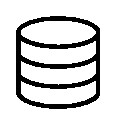
\includegraphics{./figs/icons/database.eps}};
  \node [scale=1,right=2cm of do](sp){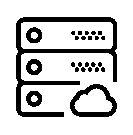
\includegraphics{./figs/icons/server.eps}};
  \node [scale=2,right=2cm of sp](client){
\includegraphics{./figs/icons/user.eps}};
  \draw[-latex] (do.east) -- (sp.west) node [midway,above,font=\scriptsize] {Data \& ADS};
  \draw[-latex,transform canvas={yshift=0.5ex}] (client.west) -- (sp.east) node [midway,above,font=\scriptsize] {Queries};
  \draw[-latex,transform canvas={yshift=-0.5ex}] (sp.east) -- (client.west) node [midway,below,font=\scriptsize] {Results \& VO};
  \node [font=\footnotesize,below=0cm of sp](sp-label){\textbf{Services Provider (SP)}};
  \node [font=\footnotesize] at (do |- sp-label) {\textbf{Data Owner (DO)}};
  \node [font=\footnotesize] at (client |- sp-label) {\textbf{Clients}};
\end{tikzpicture}

        \caption{System Model}
      \end{figure}
    \item \textcolor{Red}{Security Threats}: SP cannot be fully trusted $\Rightarrow$ Query result integrity not guaranteed
    \item \textcolor{Green}{Solution}:
      \begin{itemize}[<1->]
        \item DO signs a well-designed \alert{\emph{authenticated data structure} (ADS)}
        \item SP constructs a cryptographic proof a.k.a.\ \alert{\emph{verifciation object} (VO)}
        \item Clients verify the correctness of the results based on VO
      \end{itemize}
  \end{itemize}
\end{frame}

\begin{frame}{Related Works}
  \begin{columns}
    \begin{column}{0.8\linewidth}
      \begin{itemize}[<+->]
        \item There are two approaches to support authenticated query processing
        \item \alert{ADS-based Solutions}
          \begin{itemize}[<1->]
            \item Designed specifically based on the computation task
            \item \makebox[.35\linewidth][l]{\textcolor{Green}{Pros}: efficient}
              \textcolor{Red}{Cons}: only work for the specific queries
            \item \textcolor{Violet}{Examples}:
              \parbox[t]{\linewidth}{%
                \strut%
                signature chaining~\cite{10.1109/ICDE.2004.1320027}, Merkle hash tree~\cite{10.1007/0-387-34805-0_21}, \\ set accumulator~\cite{10.1145/2660267.2660373}, etc.%
                \strut%
              }%
          \end{itemize}
        \item \alert{General-Purpose Solutions}
          \begin{itemize}[<1->]
            \item Modeling computation task as boolean or arithmetic circuit
            \item \makebox[.35\linewidth][l]{\textcolor{Green}{Pros}: expressive}
              \textcolor{Red}{Cons}: high setup \& proving cost
            \item \textcolor{Violet}{Examples}: zkSNARKs~\cite{10.1109/sp.2013.47}, RAM-based VC~\cite{10.1145/2517349.2522733}, etc.
          \end{itemize}
        \item We focus on \alert{ADS-based solutions} in this thesis
      \end{itemize}
    \end{column}%
    \begin{column}{0.2\linewidth}
      \begin{figure}
        \onslide<2->{%
          \resizebox{\linewidth}{!}{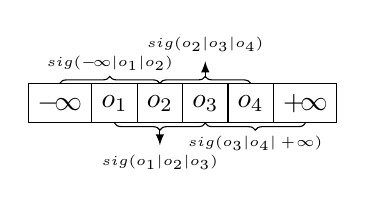
\begin{tikzpicture}
    \tikzstyle{chain-node}=[
        rectangle split,
        rectangle split horizontal,
        rectangle split ignore empty parts,
        rectangle split parts=6,
        draw
    ]
    \node[chain-node] (chain) {
        \nodepart{one} $-\!\infty$
        \nodepart{two} $o_1$
        \nodepart{three} $o_2$
        \nodepart{four} $o_3$
        \nodepart{five} $o_4$
        \nodepart{six} $+\!\infty$
    };

    \draw[decorate, decoration={brace}]
    (chain.one north) -- coordinate (s1) (chain.three north);
    \node[above=1pt of s1,font=\tiny] (s1-label) {$sig(-\!\infty|o_1|o_2)$};

    \draw[decorate, decoration={brace,mirror}]
    (chain.two south) -- coordinate[below=2pt] (s2) (chain.four south);
    \node[below=6pt of s2,font=\tiny] (s2-label) {$sig(o_1|o_2|o_3)$};
    \draw[-latex] (s2) -- (s2-label);

    \draw[decorate, decoration={brace}]
    (chain.three north) -- coordinate[above=2pt] (s3) (chain.five north);
    \node[above=6pt of s3,font=\tiny] (s3-label) {$sig(o_2|o_3|o_4)$};
    \draw[-latex] (s3) -- (s3-label);

    \draw[decorate, decoration={brace,mirror}]
    (chain.four south) -- coordinate (s4) (chain.six south);
    \node[below=1pt of s4,font=\tiny] (s4-label) {$sig(o_3|o_4|+\!\infty)$};
\end{tikzpicture}
}
          \caption{Signature Chaining}
          \resizebox{\linewidth}{!}{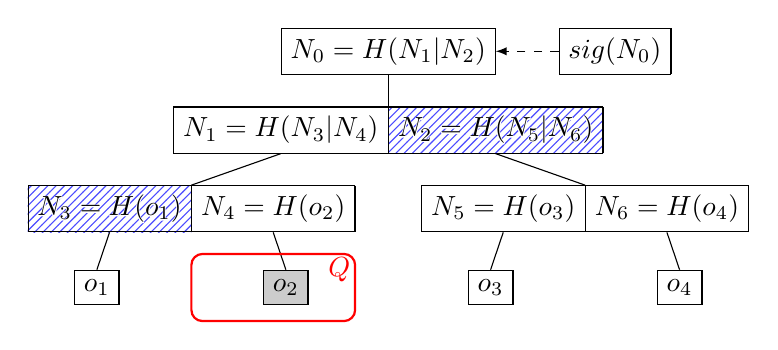
\begin{tikzpicture}
    \tikzstyle{tree node}=[
        rectangle split,
        rectangle split horizontal,
        rectangle split ignore empty parts,
        draw
    ]
    \tikzstyle{tree}=[
        every node/.style={tree node},
        edge from parent path={},
        level/.style={level distance=1cm},
        level 2/.style={sibling distance=5cm},
        level 3/.style={sibling distance=2.4cm},
    ]

    \path[tree] node (root) {$N_0 = H(N_1|N_2)$}
    child {
        node (l1) {
            \nodepart{one} $N_1 = H(N_3|N_4)$ \nodepart{two} \contour{white}{$N_2 = H(N_5|N_6)$}
        }
        child {
            node (l21) {
                \nodepart{one} \contour{white}{$N_3 = H(o_1)$} \nodepart{two} $N_4 = H(o_2)$
            }
            child {node (o1) {$o_1$}}
            child {node [fill=black!20, text=black] (o2) {$o_2$}}
        }
        child {
            node (l22) {
                \nodepart{one} $N_5 = H(o_3)$ \nodepart{two} $N_6 = H(o_4)$
            }
            child {node (o3) {$o_3$}}
            child {node (o4) {$o_4$}}
        }
    };

    \begin{pgfonlayer}{background}
        \fill[pattern=north east lines,pattern color=blue!70]
        (l21.north west) rectangle (l21.one split south);
        \fill[pattern=north east lines,pattern color=blue!70]
        (l1.one split north) rectangle (l1.south east);
    \end{pgfonlayer}

    \foreach \a/\b in {
        root.south/l1,
        l1.one south/l21,
        l1.two south/l22,
        l21.one south/o1,
        l21.two south/o2,
        l22.one south/o3,
        l22.two south/o4%
    }
    \draw [style=edge from parent] (\a) -- (\b.north);

    \node[tree node,right=0.8cm of root] (data) {$sig(N_0)$};
    \draw[dashed,-latex] (data) -- (root);

    \draw [Red,rounded corners,thick]
    let \p1 = ($(o2.south east -| l21.one split) - (0, 0.2)$),
    \p2 = ($(o2.north west -| l21.east) + (0, 0.2)$) in
    (\x1, \y1) rectangle (\x2, \y2)
    node[xshift=-0.2cm, yshift=-0.2cm] {$Q$};
\end{tikzpicture}
}
          \caption{Merkle Hash Tree}
          \onslide<3->{%
            \resizebox{\linewidth}{!}{\begin{tikzpicture}
  \node[matrix] (circuit) {
    \node (circuit-fig) {%
      \begin{tikzpicture}[scale=0.2]
        \node[circle,draw=black,minimum size=10,inner sep=0] (g1) at (0, 0) {};
        \node[circle,draw=black,minimum size=10,inner sep=0] (g2) at (-1, 2) {};
        \node[circle,draw=black,minimum size=10,inner sep=0] (g3) at (1, 2) {};
        \draw (g1) -- (0, -1.5);
        \draw (g1) -- (g2);
        \draw (g1) -- (g3);
        \draw (g2) -- (-0.25, 4);
        \draw (g2) -- (-2, 4);
        \draw (g3) -- (0.25, 4);
        \draw (g3) -- (2, 4);
      \end{tikzpicture}
    };
    \node[below=0cm of circuit-fig] {Circuit};
    \\
  };

  \node[matrix, left=0.2cm of circuit] (input) {
    \node (db) {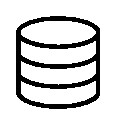
\includegraphics[width=0.6cm]{./figs/icons/database.eps}};
    \node[left=0cm of db] {Data};
    \node[below=0.6cm of db] (sql) {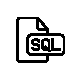
\includegraphics[width=0.6cm]{./figs/icons/sql.eps}};
    \node[left=0cm of sql] {Program};
    \draw[decorate,decoration={brace,amplitude=10pt}]
    (db.east) -- coordinate[right=10pt] (input-mid) (sql.east);
    \\
  };
  \draw[-latex] (input-mid) -- (circuit);

  \node[matrix,right=0.5cm of circuit] (proof) {
    \node (cert) {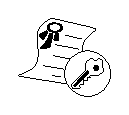
\includegraphics[width=0.7cm]{./figs/icons/cert.eps}};
    \node[below=0cm of cert] {Proof};
    \\
  };
  \draw[-latex] (circuit) -- (proof);
\end{tikzpicture}
}
            \caption{zkSNARKs}
          }
        }
      \end{figure}%
    \end{column}
  \end{columns}
\end{frame}

\begin{frame}{Related Works}
  \begin{itemize}[<+->]
    \item However, the prior works have only considered \alert{limited query types}
    \item They fail to consider:
      \begin{itemize}[<+- | alert@+>]
        \item Aggregate queries over set-valued data for data analytics
        \item Enforcing fine-grained access control
        \item Query processing in distributed settings
      \end{itemize}
  \end{itemize}

  \begin{columns}[b]
    \begin{column}{0.33\linewidth}
      \begin{figure}
        \onslide<3->{%
          \resizebox{\linewidth}{!}{\begin{tikzpicture}
  \node[matrix,ampersand replacement=\&] (input) {
    \node (data) {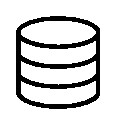
\includegraphics[width=0.5cm]{./figs/icons/database.eps}};
    \node[right=0 of data,scale=0.5] (table) {
      \begin{tabular}{|l|l|}
        \hline
        $o_1$ & $\{a, b, c\}$ \\
        \hline
        $o_2$ & $\{a, d\}$ \\
        \hline
        $\cdots$ & $\cdots$ \\
        \hline
      \end{tabular}
    };
    \\
  };
  \node[right=0.5cm of input] (out) {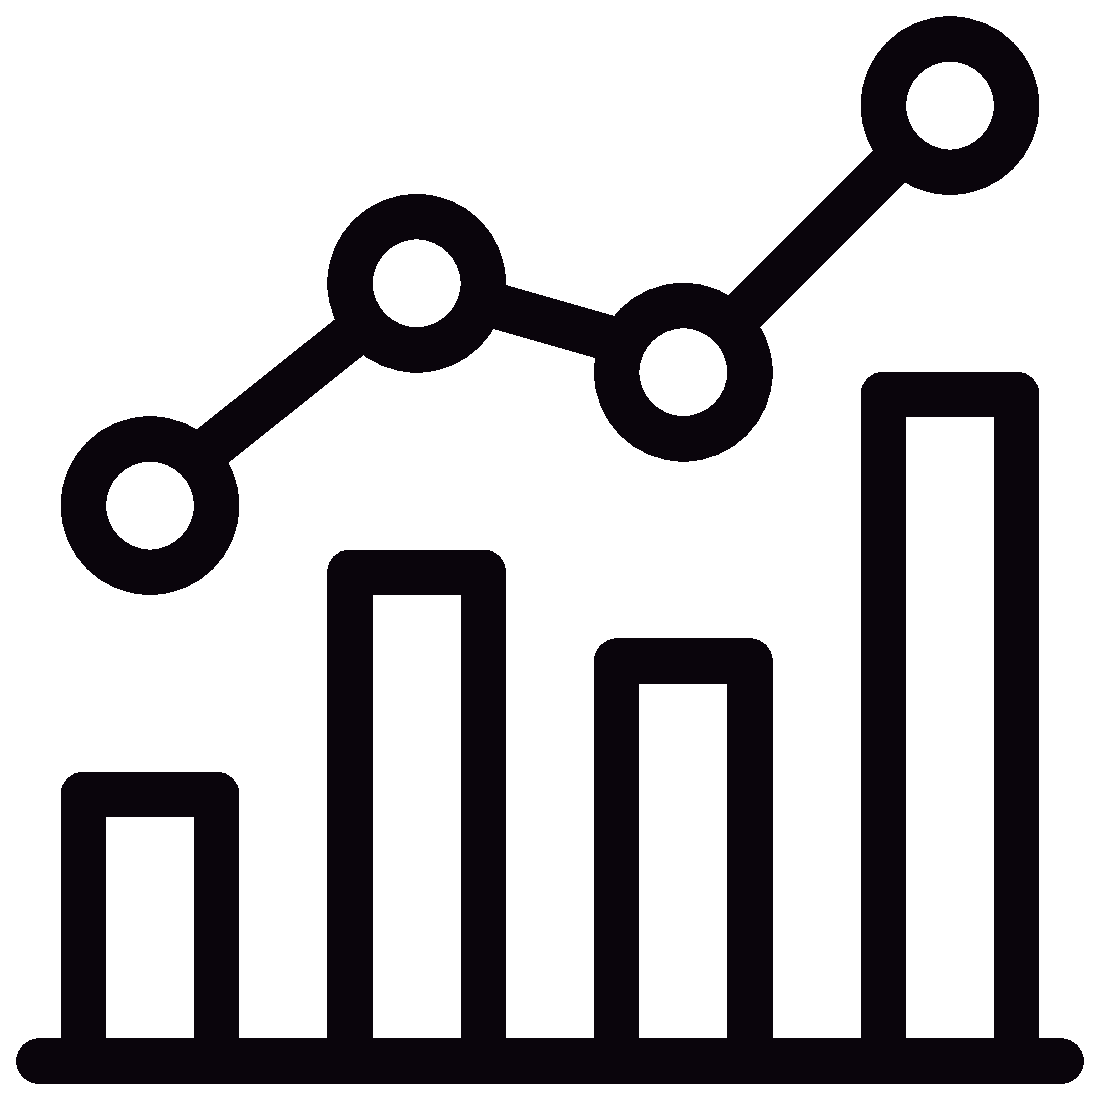
\includegraphics[width=0.5cm]{./figs/icons/analytics.eps}};
  \draw[-latex] (input) -- (out);
\end{tikzpicture}
}
          \caption{Analytical Queries}
        }
      \end{figure}
    \end{column}
    \begin{column}{0.33\linewidth}
      \begin{figure}
        \onslide<4->{%
          \resizebox{\linewidth}{!}{\begin{tikzpicture}
  \node[matrix, inner sep=0] (output) {
    \node[scale=0.9] at (0,0.5) (user1) {
\includegraphics{figs/icons/user.eps}};
    \node[scale=0.9] at (0,-0.5) (user2) {
\includegraphics{figs/icons/user.eps}};
    \node[right=0cm of user1] (user1-info) {$u_1: \{Role_A, Role_B\}$};
    \node[right=0cm of user2] (user2-info) {$u_2: \{Role_C\}$};
    \\
  };

  \coordinate (user-mid) at ($(user1)!.5!(user2)$);
  \node[left=2cm of user-mid] (input) {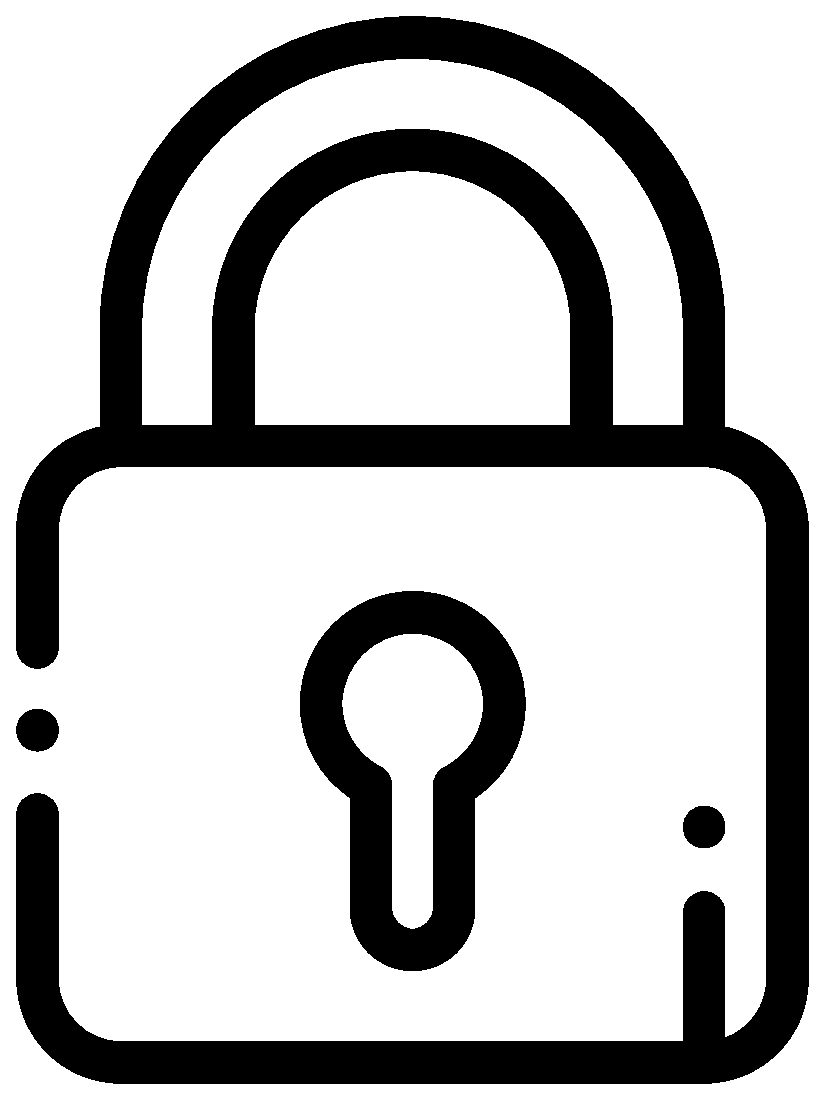
\includegraphics[width=0.5cm]{figs/icons/lock.eps}};
  \node[below=0cm of input] {$\Upsilon = Role_A $};
  \coordinate (mid) at ($(input)!.4!(user-mid)$);
  \draw (input.east) -- (mid);
  \draw[-latex] (mid) |- (user1.west) node[pos=0.75, sloped, scale=1, color=Green] {\ding{52}};
  \draw[-latex] (mid) |- (user2.west) node[pos=0.75, sloped, scale=1, color=Red] {\ding{55}};
\end{tikzpicture}
}
          \caption{Access Control}
        }
      \end{figure}
    \end{column}
    \begin{column}{0.33\linewidth}
      \begin{figure}
        \onslide<5->{%
          \resizebox{\linewidth}{!}{\begin{tikzpicture}
  \node[matrix,inner sep=0.01cm,draw=black,ellipse,dashed] (server) {%
    \node (s1) {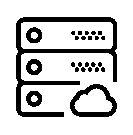
\includegraphics[width=0.5cm]{./figs/icons/server.eps}};
    \node[below=0 of s1.south east, anchor=north west] (s2) {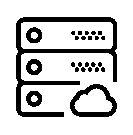
\includegraphics[width=0.5cm]{./figs/icons/server.eps}};
    \node[below=0 of s1.south west, anchor=north east] (s3) {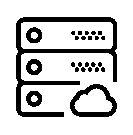
\includegraphics[width=0.5cm]{./figs/icons/server.eps}};
    \\
  };

  \node[scale=0.9,left=2cm of server] (user) {
\includegraphics{./figs/icons/user.eps}};
  \draw[-latex] (user) -- (server) node[midway, above, color=Red] {$q: \langle k, loc \rangle$};
\end{tikzpicture}
}
          \caption{Distributed Query Processing}
        }
      \end{figure}
    \end{column}
  \end{columns}
\end{frame}

\section{Authenticating Aggregate Queries over Set-Valued Data}

\begin{frame}[fragile]{Example of Aggregate Queries over Set-Valued Data}
  \begin{columns}
    \begin{column}{.5\linewidth}
      \setbeamercovered{transparent}
      \begin{table}
        \resizebox{\linewidth}{!}{%
          \begin{tabular}{ccl}
            \toprule
            \textbf{PID} & \textbf{ZIP} & \multicolumn{1}{c}{\textbf{Mut-Genes}}\\
            \midrule
            \onslide<1,2,3>{P1&95014&\alert<2>{A-C130R}, P-I696M} \\
            \onslide<1,3,4>{P2&20482&H-C282Y, \alert<4>{P-P12A}, \alert<3,4>{R-G1886S}} \\
            \onslide<1,2,3>{P3&95014&\alert<2>{A-C130R}, U-G71R, W-R611H} \\
            \onslide<1,3>{P4&01720&A-V2050L, H-C282Y, M-R52C, U-G71R} \\
            \onslide<1,3,4>{P5&20134&A-C130R, \alert<4>{P-P12A}, \alert<3,4>{R-G1886S}, S-E366K} \\
            \onslide<1,3>{P6&17868& C-R102G, \alert<3>{R-G1886S}} \\
            \onslide<1,3>{P7&55410&C-R102G, C-Q1334H, S-E288V} \\
            \onslide<1,3,4>{P8&20852&C-R102G, \alert<4>{P-P12A}, \alert<3,4>{R-G1886S}, K-T220M} \\
            \bottomrule
          \end{tabular}
        }
        \caption{Set-Valued Genome Dataset~\cite{pgp}}
      \end{table}
    \end{column}%
    \begin{column}{.5\linewidth}
      \begin{itemize}[<+(1)->]
        \item \textbf{Q1}: Find the most common gene in the district of Cupertino, CA (ZIP\@: 95014) \\
          \textcolor{Violet}{\emph{Answer:} \{`A-C130R'\}}
        \item \textbf{Q2}: Count the number of participants who carry the gene `R-G1886S' \\
          \textcolor{Violet}{\emph{Answer:} 4}
        \item \textbf{Q3}: Find the most frequent genes with supports $\ge$ 3 in ZIPs 20*** \\
          \textcolor{Violet}{\emph{Answer:} \{`P-P12A', `R-G1886S'\}}
      \end{itemize}
    \end{column}
  \end{columns}
\end{frame}

\begin{frame}{Problem Definition}
  \begin{itemize}[<+->]
    \item \textbf{Dataset} $\mathbb{D} = \{o_1, o_2, \dots, o_n\}$
      \begin{itemize}[<.->]
        \item $o_i = \langle A_i, X_i \rangle$.
        \item $A_i$ is a set of \textcolor{Green}{non-sensitive} attributes
        \item $X_i$ is a \textcolor{Red}{sensitive} multiset of \emph{features}
      \end{itemize}
    \item \textbf{Aggregate Query} $Q = (q, \{x_i\}, [\alpha, \beta])$
      \begin{itemize}[<.->]
        \item $q$ is an aggregate operator, i.e., \emph{max/min}, \emph{count}, \emph{sum}, \emph{top-$k$}, and \emph{frequent feature query (FFQ)}
        \item $\{x_i\}$ is the queried feature specified for \emph{count} and \emph{sum}
        \item $[\alpha, \beta]$ specifies the selection range over the \textcolor{Green}{non-sensitive} attributes
      \end{itemize}
    \item \textbf{Threat Model}
      \begin{itemize}[<.->]
        \item \alert{Integrity}: SP should prove the \emph{soundness} and \emph{completeness} of the results
        \item \alert{Confidentiality}: Clients should not infer any \emph{sensitive source data}
      \end{itemize}
  \end{itemize}
\end{frame}

\begin{frame}{Preliminaries}
  \begin{definition}<+->[Bilinear-Map (BM) Accumulator]
    Let $g$ be the group generator of a cyclic multiplicative group $\mathbb{G}$ and $s$ be a \textcolor{Red}{private value of DO}. The accumulator maps a multiset $X = \{ x_1, x_2, \dotsc, x_m \}$ to a single value in $\mathbb{G}$:
    \begin{align*}
      acc(X) = g^{P(X)} = g^{\prod_{x_i \in X}(x_i + s)}
    \end{align*}
    Without knowing $s$, one can still compute an $acc(\cdot)$ value by giving $g^s, g^{s^2}, \dotsc$
  \end{definition}
  \begin{example}<+->
    $X = \{ 1, 1, 2 \}$, $acc(X) = g^{(1+s)^2(2+s)} = g^{s^3+4 s^2+5 s+2} = g^{s^3} \cdot (g^{s^2})^4 \cdot(g^s)^5 \cdot g^2$
  \end{example}
  \begin{definition}<+->[Randomized BM Accumulator]
    BM accumulator is \alert{deterministic} for \emph{a fixed multiset}. As such, an adversary can tell in high confidence that two multisets are the same. We can randomize BM accumulator as following:
    \begin{align*}
      acc(X) = g^{P(X) \cdot r_X} = g^{r_X\prod_{x_i \in X}(x_i + s)}
    \end{align*}
    $r_X$ is a random value \textcolor{Red}{hidden from Clients} but \textcolor{Green}{disclosed to SP}
  \end{definition}
\end{frame}

\begin{frame}{Preliminaries}
  \begin{definition}[Cryptographic Hash Function]
    A cryptographic hash function $H(\cdot)$ accepts an arbitrary-length string as its input and returns a fixed-length bit string such that it is computationally infeasible to find $m_1 \neq m_2$ and $H(m_1) = H(m_2)$.
  \end{definition}
  \begin{definition}[Bilinear Pairing]
    Let $\mathbb{G}, \mathbb{G}_T$ be two cyclic multiplicative groups of order $p$.
    A pairing is a map $e: \mathbb{G} \times \mathbb{G} \to \mathbb{G}_T$, which satisfies:
    \begin{itemize}
      \item \textbf{Bilinearity}: $e(u^a,v^b) = {e(u,v)}^{ab}$, $\forall u, v \in \mathbb{G}$
      \item \textbf{Non-degeneracy}: $e(g,g) \ne 1$
      \item \textbf{Computability}: Given $u, v \in \mathbb{G}$, it is easy to compute $e(u, v)$
    \end{itemize}
  \end{definition}
\end{frame}

\begin{frame}[fragile]{PA$^2$ Authentication Framework Overview}
  \begin{figure}
    \onslide<+->{%
      \resizebox{.8\linewidth}{!}{%
        \begin{tikzpicture}
          \node[anchor=south west,inner sep=0] (A) at (0,0)
            {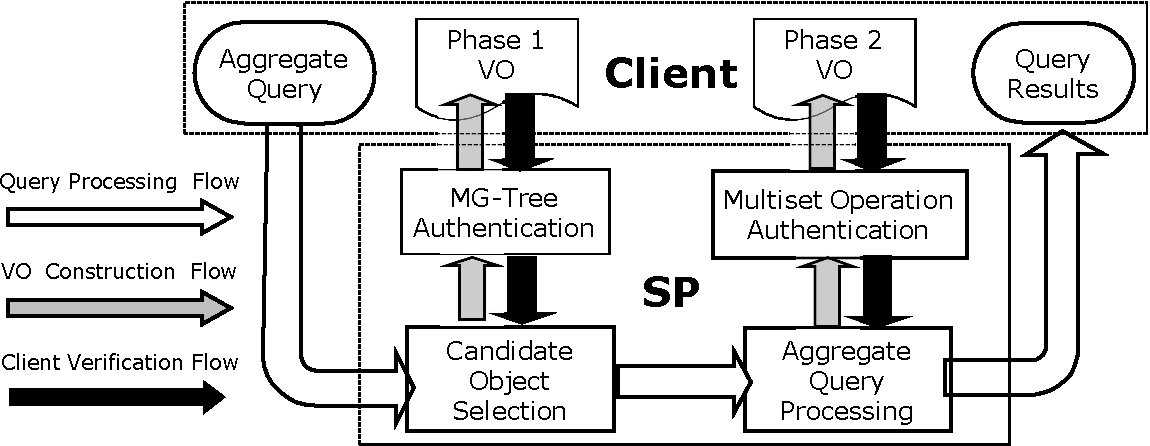
\includegraphics[width=\linewidth]{figs/aggregate-queries/overview.pdf}};
          \coordinate (multiset1) at (8.6,2.2);
          \coordinate (multiset2) at (11.9,3.45);
          \coordinate (aggregate1) at (9,0.1);
          \coordinate (aggregate2) at (11.7,1.55);
          \coordinate (select1) at (4.8,0.1);
          \coordinate (select2) at (7.57,3.45);
          \draw<2>[Red,ultra thick] (multiset1) rectangle (multiset2);
          \fill<2>[draw=none,fill=black,fill opacity=0.3,even odd rule]
            (A.south west) rectangle (A.north east)
            (multiset1) rectangle (multiset2);
          \draw<3>[Red,ultra thick] (aggregate1) rectangle (aggregate2);
          \fill<3>[draw=none,fill=black,fill opacity=0.3,even odd rule]
            (A.south west) rectangle (A.north east)
            (aggregate1) rectangle (aggregate2);
          \draw<4>[Red,ultra thick] (select1) rectangle (select2);
          \fill<4>[draw=none,fill=black,fill opacity=0.3,even odd rule]
            (A.south west) rectangle (A.north east)
            (select1) rectangle (select2);
        \end{tikzpicture}
      }
      \caption{Privacy-Preserving Authentication Framework for Aggregate Queries}
    }
  \end{figure}
  \begin{itemize}[<+- | alert@+>]
    \item PA$^2$ Protocols on Multiset Operations
    \item PA$^2$ Algorithms on Aggregate Queries
    \item PA$^2$ on Candidate Object Selection
  \end{itemize}
\end{frame}

\section{Authenticating Relational Queries with Fine-Grained Access Control}

\section{Authenticating {kNN} Queries in Distributed Settings}

\section{Conclusions}

\begin{frame}[standout]
  Thanks \\
  Questions?
\end{frame}

\appendix%

\begingroup
\setbeamertemplate{frametitle continuation}{}
\begin{frame}[t,allowframebreaks]{\refname}
  \bookmark[page=\thepage,startatroot]{\refname}
  \setbeamertemplate{bibliography item}[text]
  \renewcommand*{\bibfont}{\scriptsize}
  \printbibliography[heading=none]%
\end{frame}
\endgroup

\end{document}
